% generated by paper/scripts/nesting_slice.py from certificates/candidate_certificate.json (children)
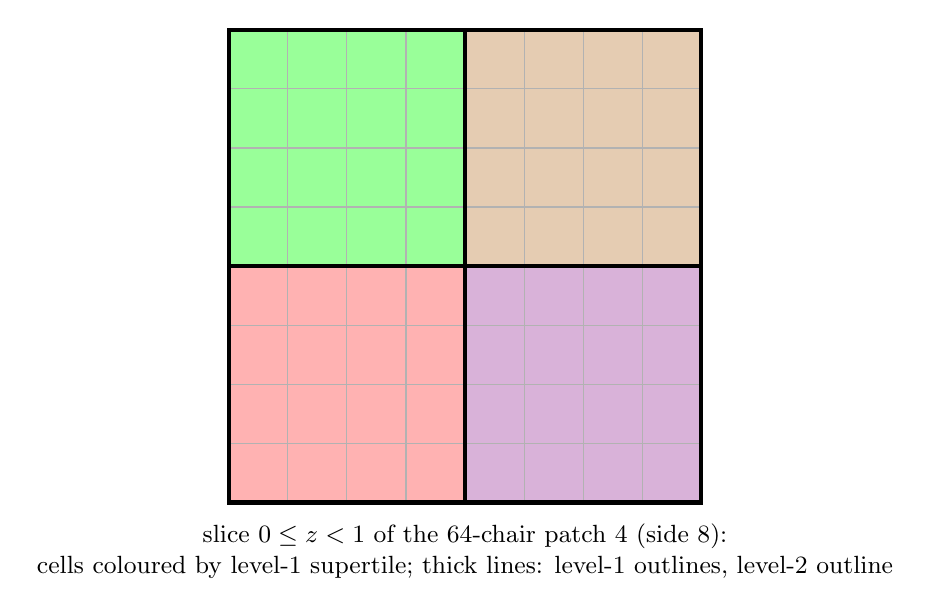
\begin{tikzpicture}[x=1cm,y=1cm,font=\scriptsize]
  \fill[red!30] (0.0,0.0) rectangle (0.75,0.75);
  \draw[gray!60,thin] (0.0,0.0) rectangle (0.75,0.75);
  \fill[red!30] (0.0,0.75) rectangle (0.75,1.5);
  \draw[gray!60,thin] (0.0,0.75) rectangle (0.75,1.5);
  \fill[red!30] (0.0,1.5) rectangle (0.75,2.25);
  \draw[gray!60,thin] (0.0,1.5) rectangle (0.75,2.25);
  \fill[red!30] (0.0,2.25) rectangle (0.75,3.0);
  \draw[gray!60,thin] (0.0,2.25) rectangle (0.75,3.0);
  \fill[green!40] (0.0,3.0) rectangle (0.75,3.75);
  \draw[gray!60,thin] (0.0,3.0) rectangle (0.75,3.75);
  \fill[green!40] (0.0,3.75) rectangle (0.75,4.5);
  \draw[gray!60,thin] (0.0,3.75) rectangle (0.75,4.5);
  \fill[green!40] (0.0,4.5) rectangle (0.75,5.25);
  \draw[gray!60,thin] (0.0,4.5) rectangle (0.75,5.25);
  \fill[green!40] (0.0,5.25) rectangle (0.75,6.0);
  \draw[gray!60,thin] (0.0,5.25) rectangle (0.75,6.0);
  \fill[red!30] (0.75,0.0) rectangle (1.5,0.75);
  \draw[gray!60,thin] (0.75,0.0) rectangle (1.5,0.75);
  \fill[red!30] (0.75,0.75) rectangle (1.5,1.5);
  \draw[gray!60,thin] (0.75,0.75) rectangle (1.5,1.5);
  \fill[red!30] (0.75,1.5) rectangle (1.5,2.25);
  \draw[gray!60,thin] (0.75,1.5) rectangle (1.5,2.25);
  \fill[red!30] (0.75,2.25) rectangle (1.5,3.0);
  \draw[gray!60,thin] (0.75,2.25) rectangle (1.5,3.0);
  \fill[green!40] (0.75,3.0) rectangle (1.5,3.75);
  \draw[gray!60,thin] (0.75,3.0) rectangle (1.5,3.75);
  \fill[green!40] (0.75,3.75) rectangle (1.5,4.5);
  \draw[gray!60,thin] (0.75,3.75) rectangle (1.5,4.5);
  \fill[green!40] (0.75,4.5) rectangle (1.5,5.25);
  \draw[gray!60,thin] (0.75,4.5) rectangle (1.5,5.25);
  \fill[green!40] (0.75,5.25) rectangle (1.5,6.0);
  \draw[gray!60,thin] (0.75,5.25) rectangle (1.5,6.0);
  \fill[red!30] (1.5,0.0) rectangle (2.25,0.75);
  \draw[gray!60,thin] (1.5,0.0) rectangle (2.25,0.75);
  \fill[red!30] (1.5,0.75) rectangle (2.25,1.5);
  \draw[gray!60,thin] (1.5,0.75) rectangle (2.25,1.5);
  \fill[red!30] (1.5,1.5) rectangle (2.25,2.25);
  \draw[gray!60,thin] (1.5,1.5) rectangle (2.25,2.25);
  \fill[red!30] (1.5,2.25) rectangle (2.25,3.0);
  \draw[gray!60,thin] (1.5,2.25) rectangle (2.25,3.0);
  \fill[green!40] (1.5,3.0) rectangle (2.25,3.75);
  \draw[gray!60,thin] (1.5,3.0) rectangle (2.25,3.75);
  \fill[green!40] (1.5,3.75) rectangle (2.25,4.5);
  \draw[gray!60,thin] (1.5,3.75) rectangle (2.25,4.5);
  \fill[green!40] (1.5,4.5) rectangle (2.25,5.25);
  \draw[gray!60,thin] (1.5,4.5) rectangle (2.25,5.25);
  \fill[green!40] (1.5,5.25) rectangle (2.25,6.0);
  \draw[gray!60,thin] (1.5,5.25) rectangle (2.25,6.0);
  \fill[red!30] (2.25,0.0) rectangle (3.0,0.75);
  \draw[gray!60,thin] (2.25,0.0) rectangle (3.0,0.75);
  \fill[red!30] (2.25,0.75) rectangle (3.0,1.5);
  \draw[gray!60,thin] (2.25,0.75) rectangle (3.0,1.5);
  \fill[red!30] (2.25,1.5) rectangle (3.0,2.25);
  \draw[gray!60,thin] (2.25,1.5) rectangle (3.0,2.25);
  \fill[red!30] (2.25,2.25) rectangle (3.0,3.0);
  \draw[gray!60,thin] (2.25,2.25) rectangle (3.0,3.0);
  \fill[green!40] (2.25,3.0) rectangle (3.0,3.75);
  \draw[gray!60,thin] (2.25,3.0) rectangle (3.0,3.75);
  \fill[green!40] (2.25,3.75) rectangle (3.0,4.5);
  \draw[gray!60,thin] (2.25,3.75) rectangle (3.0,4.5);
  \fill[green!40] (2.25,4.5) rectangle (3.0,5.25);
  \draw[gray!60,thin] (2.25,4.5) rectangle (3.0,5.25);
  \fill[green!40] (2.25,5.25) rectangle (3.0,6.0);
  \draw[gray!60,thin] (2.25,5.25) rectangle (3.0,6.0);
  \fill[violet!30] (3.0,0.0) rectangle (3.75,0.75);
  \draw[gray!60,thin] (3.0,0.0) rectangle (3.75,0.75);
  \fill[violet!30] (3.0,0.75) rectangle (3.75,1.5);
  \draw[gray!60,thin] (3.0,0.75) rectangle (3.75,1.5);
  \fill[violet!30] (3.0,1.5) rectangle (3.75,2.25);
  \draw[gray!60,thin] (3.0,1.5) rectangle (3.75,2.25);
  \fill[violet!30] (3.0,2.25) rectangle (3.75,3.0);
  \draw[gray!60,thin] (3.0,2.25) rectangle (3.75,3.0);
  \fill[brown!40] (3.0,3.0) rectangle (3.75,3.75);
  \draw[gray!60,thin] (3.0,3.0) rectangle (3.75,3.75);
  \fill[brown!40] (3.0,3.75) rectangle (3.75,4.5);
  \draw[gray!60,thin] (3.0,3.75) rectangle (3.75,4.5);
  \fill[brown!40] (3.0,4.5) rectangle (3.75,5.25);
  \draw[gray!60,thin] (3.0,4.5) rectangle (3.75,5.25);
  \fill[brown!40] (3.0,5.25) rectangle (3.75,6.0);
  \draw[gray!60,thin] (3.0,5.25) rectangle (3.75,6.0);
  \fill[violet!30] (3.75,0.0) rectangle (4.5,0.75);
  \draw[gray!60,thin] (3.75,0.0) rectangle (4.5,0.75);
  \fill[violet!30] (3.75,0.75) rectangle (4.5,1.5);
  \draw[gray!60,thin] (3.75,0.75) rectangle (4.5,1.5);
  \fill[violet!30] (3.75,1.5) rectangle (4.5,2.25);
  \draw[gray!60,thin] (3.75,1.5) rectangle (4.5,2.25);
  \fill[violet!30] (3.75,2.25) rectangle (4.5,3.0);
  \draw[gray!60,thin] (3.75,2.25) rectangle (4.5,3.0);
  \fill[brown!40] (3.75,3.0) rectangle (4.5,3.75);
  \draw[gray!60,thin] (3.75,3.0) rectangle (4.5,3.75);
  \fill[brown!40] (3.75,3.75) rectangle (4.5,4.5);
  \draw[gray!60,thin] (3.75,3.75) rectangle (4.5,4.5);
  \fill[brown!40] (3.75,4.5) rectangle (4.5,5.25);
  \draw[gray!60,thin] (3.75,4.5) rectangle (4.5,5.25);
  \fill[brown!40] (3.75,5.25) rectangle (4.5,6.0);
  \draw[gray!60,thin] (3.75,5.25) rectangle (4.5,6.0);
  \fill[violet!30] (4.5,0.0) rectangle (5.25,0.75);
  \draw[gray!60,thin] (4.5,0.0) rectangle (5.25,0.75);
  \fill[violet!30] (4.5,0.75) rectangle (5.25,1.5);
  \draw[gray!60,thin] (4.5,0.75) rectangle (5.25,1.5);
  \fill[violet!30] (4.5,1.5) rectangle (5.25,2.25);
  \draw[gray!60,thin] (4.5,1.5) rectangle (5.25,2.25);
  \fill[violet!30] (4.5,2.25) rectangle (5.25,3.0);
  \draw[gray!60,thin] (4.5,2.25) rectangle (5.25,3.0);
  \fill[brown!40] (4.5,3.0) rectangle (5.25,3.75);
  \draw[gray!60,thin] (4.5,3.0) rectangle (5.25,3.75);
  \fill[brown!40] (4.5,3.75) rectangle (5.25,4.5);
  \draw[gray!60,thin] (4.5,3.75) rectangle (5.25,4.5);
  \fill[brown!40] (4.5,4.5) rectangle (5.25,5.25);
  \draw[gray!60,thin] (4.5,4.5) rectangle (5.25,5.25);
  \fill[brown!40] (4.5,5.25) rectangle (5.25,6.0);
  \draw[gray!60,thin] (4.5,5.25) rectangle (5.25,6.0);
  \fill[violet!30] (5.25,0.0) rectangle (6.0,0.75);
  \draw[gray!60,thin] (5.25,0.0) rectangle (6.0,0.75);
  \fill[violet!30] (5.25,0.75) rectangle (6.0,1.5);
  \draw[gray!60,thin] (5.25,0.75) rectangle (6.0,1.5);
  \fill[violet!30] (5.25,1.5) rectangle (6.0,2.25);
  \draw[gray!60,thin] (5.25,1.5) rectangle (6.0,2.25);
  \fill[violet!30] (5.25,2.25) rectangle (6.0,3.0);
  \draw[gray!60,thin] (5.25,2.25) rectangle (6.0,3.0);
  \fill[brown!40] (5.25,3.0) rectangle (6.0,3.75);
  \draw[gray!60,thin] (5.25,3.0) rectangle (6.0,3.75);
  \fill[brown!40] (5.25,3.75) rectangle (6.0,4.5);
  \draw[gray!60,thin] (5.25,3.75) rectangle (6.0,4.5);
  \fill[brown!40] (5.25,4.5) rectangle (6.0,5.25);
  \draw[gray!60,thin] (5.25,4.5) rectangle (6.0,5.25);
  \fill[brown!40] (5.25,5.25) rectangle (6.0,6.0);
  \draw[gray!60,thin] (5.25,5.25) rectangle (6.0,6.0);
  \draw[very thick] (0.0,0.0) -- (0.0,0.75);
  \draw[very thick] (0.0,0.0) -- (0.75,0.0);
  \draw[very thick] (0.0,0.75) -- (0.0,1.5);
  \draw[very thick] (0.75,0.0) -- (1.5,0.0);
  \draw[very thick] (0.0,2.25) -- (0.0,3.0);
  \draw[very thick] (0.0,3.0) -- (0.75,3.0);
  \draw[very thick] (0.0,1.5) -- (0.0,2.25);
  \draw[very thick] (0.75,3.0) -- (1.5,3.0);
  \draw[very thick] (3.0,0.0) -- (3.0,0.75);
  \draw[very thick] (2.25,0.0) -- (3.0,0.0);
  \draw[very thick] (1.5,0.0) -- (2.25,0.0);
  \draw[very thick] (3.0,0.75) -- (3.0,1.5);
  \draw[very thick] (3.0,2.25) -- (3.0,3.0);
  \draw[very thick] (2.25,3.0) -- (3.0,3.0);
  \draw[very thick] (3.0,1.5) -- (3.0,2.25);
  \draw[very thick] (1.5,3.0) -- (2.25,3.0);
  \draw[very thick] (0.0,5.25) -- (0.0,6.0);
  \draw[very thick] (0.0,6.0) -- (0.75,6.0);
  \draw[very thick] (0.0,4.5) -- (0.0,5.25);
  \draw[very thick] (0.75,6.0) -- (1.5,6.0);
  \draw[very thick] (0.0,3.0) -- (0.0,3.75);
  \draw[very thick] (0.0,3.0) -- (0.75,3.0);
  \draw[very thick] (0.0,3.75) -- (0.0,4.5);
  \draw[very thick] (0.75,3.0) -- (1.5,3.0);
  \draw[very thick] (3.0,5.25) -- (3.0,6.0);
  \draw[very thick] (2.25,6.0) -- (3.0,6.0);
  \draw[very thick] (1.5,6.0) -- (2.25,6.0);
  \draw[very thick] (3.0,4.5) -- (3.0,5.25);
  \draw[very thick] (3.0,3.0) -- (3.0,3.75);
  \draw[very thick] (2.25,3.0) -- (3.0,3.0);
  \draw[very thick] (1.5,3.0) -- (2.25,3.0);
  \draw[very thick] (3.0,3.75) -- (3.0,4.5);
  \draw[very thick] (6.0,0.0) -- (6.0,0.75);
  \draw[very thick] (5.25,0.0) -- (6.0,0.0);
  \draw[very thick] (4.5,0.0) -- (5.25,0.0);
  \draw[very thick] (6.0,0.75) -- (6.0,1.5);
  \draw[very thick] (3.0,0.0) -- (3.0,0.75);
  \draw[very thick] (3.0,0.0) -- (3.75,0.0);
  \draw[very thick] (3.75,0.0) -- (4.5,0.0);
  \draw[very thick] (3.0,0.75) -- (3.0,1.5);
  \draw[very thick] (6.0,2.25) -- (6.0,3.0);
  \draw[very thick] (5.25,3.0) -- (6.0,3.0);
  \draw[very thick] (6.0,1.5) -- (6.0,2.25);
  \draw[very thick] (4.5,3.0) -- (5.25,3.0);
  \draw[very thick] (3.0,2.25) -- (3.0,3.0);
  \draw[very thick] (3.0,3.0) -- (3.75,3.0);
  \draw[very thick] (3.75,3.0) -- (4.5,3.0);
  \draw[very thick] (3.0,1.5) -- (3.0,2.25);
  \draw[very thick] (6.0,5.25) -- (6.0,6.0);
  \draw[very thick] (5.25,6.0) -- (6.0,6.0);
  \draw[very thick] (6.0,4.5) -- (6.0,5.25);
  \draw[very thick] (4.5,6.0) -- (5.25,6.0);
  \draw[very thick] (6.0,3.0) -- (6.0,3.75);
  \draw[very thick] (5.25,3.0) -- (6.0,3.0);
  \draw[very thick] (6.0,3.75) -- (6.0,4.5);
  \draw[very thick] (4.5,3.0) -- (5.25,3.0);
  \draw[very thick] (3.0,5.25) -- (3.0,6.0);
  \draw[very thick] (3.0,6.0) -- (3.75,6.0);
  \draw[very thick] (3.75,6.0) -- (4.5,6.0);
  \draw[very thick] (3.0,4.5) -- (3.0,5.25);
  \draw[very thick] (3.0,3.0) -- (3.0,3.75);
  \draw[very thick] (3.0,3.0) -- (3.75,3.0);
  \draw[very thick] (3.0,3.75) -- (3.0,4.5);
  \draw[very thick] (3.75,3.0) -- (4.5,3.0);
  \draw[line width=1.6pt,black] (0,0) rectangle (6.0,6.0);
  \node[anchor=north,font=\small,align=center] at (3.0,-0.15) {slice $0\le z<1$ of the $64$-chair patch $4\carrier$ (side $8$):\\ cells coloured by level-1 supertile; thick lines: level-1 outlines, level-2 outline};
\end{tikzpicture}
